\documentclass[11pt,twoside]{article}

\usepackage[margin=1in]{geometry}
\usepackage{amsmath,amssymb,amsthm,mathtools}
\usepackage[inline,shortlabels]{enumitem}
\usepackage{xcolor}
\usepackage{../misc_files/course-definition-boxes}
\usepackage{microtype}
\usepackage{array,booktabs,needspace}
\usepackage{tikz}
\usetikzlibrary{arrows.meta,positioning}
\usepackage{../exercises/course-exercises}

% Revision date: maintained by scripts/build_lecture_notes.py.
\newcommand{\lecturerevised}{2026-11-08 15:30 UTC+01:00}
\usepackage{eso-pic}
\AddToShipoutPictureBG{%
  \AtPageLowerLeft{%
    \put(\LenToUnit{0.5\paperwidth},\LenToUnit{0.5in}){%
      \makebox(0,0){\normalfont\footnotesize\color{black!60}Last revised: \lecturerevised}%
    }%
  }%
}
\usepackage[square,authoryear]{natbib}
\usepackage[colorlinks=true,linkcolor=blue!60!black,
  urlcolor=blue!60!black,citecolor=blue!60!black]{hyperref}
\usepackage[nameinlink,capitalize]{cleveref}
\crefname{exercise}{Exercise}{Exercises}
\Crefname{exercise}{Exercise}{Exercises}
\usepackage{enotez}
\DeclareInstance{enotez-list}{lecture}{list}{format=\normalsize,number={#1.}}
\setenotez{list-name=Endnotes,list-style=lecture,backref=true}
\crefname{endnote}{Endnote}{Endnotes}
\Crefname{endnote}{Endnote}{Endnotes}

\definecolor{courseblue}{HTML}{17365D}
\newcommand{\E}{\mathbb E}
\newcommand{\I}{\mathbb I}
\renewcommand{\P}{\mathbb P}
\newcommand{\R}{\mathbb R}
\newcommand{\KL}{D}
\newcommand{\TV}{\mathrm{TV}}
\makeatletter
\@for\@letter:=A,B,C,D,E,F,G,H,I,J,K,L,M,N,O,P,Q,R,S,T,U,V,W,X,Y,Z\do{%
  \expandafter\edef\csname c\@letter\endcsname{\noexpand\mathcal{\@letter}}}
\makeatother
\newcommand{\lecturenumber}{18}
\newtheorem{theorem}{Theorem}[section]
\newtheorem{proposition}[theorem]{Proposition}
\newtheorem{corollary}[theorem]{Corollary}
\newtheorem{lemma}[theorem]{Lemma}
\theoremstyle{definition}
\newtheorem{definition}[theorem]{Definition}
\newtheorem{example}[theorem]{Example}
\theoremstyle{remark}
\newtheorem{remark}[theorem]{Remark}
\renewcommand{\thepage}{\lecturenumber--\arabic{page}}
\renewcommand{\thesection}{\lecturenumber.\arabic{section}}
\renewcommand{\theequation}{\lecturenumber.\arabic{equation}}
\pagestyle{myheadings}
\markboth{Lecture 18: Imitation and reinforcement learning}
{Lecture 18: Imitation and reinforcement learning}
\hypersetup{pdftitle={Lecture 18: Imitation and reinforcement learning: the value of interaction},
  pdfauthor={Csaba Szepesvari}}

\begin{document}
\begin{center}
\fcolorbox{courseblue}{white}{%
\begin{minipage}{0.92\textwidth}
\vspace{1mm}
\textbf{CMPUT 654: Mathematical Foundations of Modern AI Systems}
\hfill Fall 2026
\vspace{3mm}
\begin{center}
{\Large\bfseries Lecture 18: Imitation and reinforcement learning\\[1mm]
The value of interaction}

\vspace{1mm}
November 3, 2026
\end{center}
\vspace{2mm}
\textit{Lecturer: Csaba Szepesv\'ari}\hfill
\textit{Notes prepared by: Csaba Szepesv\'ari}
\vspace{1mm}
\end{minipage}}
\end{center}

Can log-loss behavior cloning avoid compounding error, and when does
interaction help? For a finite policy class containing a stochastic teacher,
analysis of complete-episode likelihood gives a cloning guarantee without an
additional horizon penalty from distribution shift. We then compare data
collection methods: selected teacher queries can save teacher actions, and a
tabular reinforcement-learning example separates adaptive from passive
collection by polynomial versus exponential sample requirements.

\noindent\textbf{Reading guide.}
We begin with language generation and the finite-horizon policy framework.
\Crefrange{sec:compounding}{sec:finite} review Lecture~4's error and likelihood
arguments in trajectory notation. \Cref{sec:information} prepares the new
comparisons in \cref{sec:interaction,sec:rl}. The main text requires
probability, KL divergence, and elementary concentration. Lecture~11's
optional policy-gradient and temporal-difference sections give related
discounted models, but the finite-horizon setup is developed here.
\Cref{app:bernoulli} and the endnotes may be skipped on a first reading.
Unlike the verification target in Lecture~17, imitation seeks to reproduce
a behavior distribution, which need not be correct on every task.

\section{Language generation as sequential decision-making}
\label{sec:language}

One way to view language generation is as acting in an environment whose
state is a growing token sequence. The initial state is the prompt; an
action selects the next token; the environment appends that token to the
state. For a fixed prompt $u$, write $sa$ for the sequence $s$ with token
$a$ appended. Sampling from the next-token model $p_\theta$ of Lecture 1
then gives
\[
 S_1=u,\qquad A_h\sim p_\theta(\cdot\mid S_h),\qquad
 S_{h+1}=S_hA_h.
\]
Here $h$ counts generated tokens after the prompt. The model supplies a
\emph{policy}: a distribution over actions at each state. The environment
transition is deterministic; the policy can be stochastic.

This representation makes language generation a special case of sequential
decision-making. We can therefore use the more general frameworks of
imitation learning and reinforcement learning to ask what different forms
of training data tell us about the behavior of the resulting model.

Training on example continuations has a teacher-copying interpretation.
The teacher is the source of those continuations: a human author, another
model, or a distribution of text-producing behaviors.
\emph{Imitation learning} is the broader problem of learning behavior from
demonstrations or other access to a teacher. \emph{Behavior cloning} is a
supervised approach: fit the teacher's actions at the states recorded in
demonstrations. With log loss, this is next-token prediction on the
teacher's prefixes. Interactive imitation can additionally request teacher
actions at states selected by the learner.

Other feedback evaluates what a generated response accomplishes.
\emph{Reinforcement learning} uses reward feedback to seek a policy with
high expected total reward. In \emph{reinforcement learning from human
feedback} (RLHF), human judgments supply the training criterion, often
through a reward model fitted to comparisons of responses. In
\emph{reinforcement learning with verifiable rewards} (RLVR), computable
checks supply rewards, for example by checking a final mathematical answer
or running generated code on test cases. Both forms of feedback support
adapting a model to the tasks users want it to perform. Demonstrations and
reward-labeled data can be collected in advance or acquired during training;
interaction determines which additional observations the learner can obtain.

\section{What is being cloned?}
\label{sec:setup}

Imitation learning estimates a policy from observations of a teacher's
behavior. To discuss distribution shift, we need to specify how a policy
generates its future inputs. To discuss a stochastic teacher, we also need
a target that compares distributions rather than particular sampled actions.

\subsection{Policies and complete trajectories}

Consider a controlled process with a finite state space $\cS$, a finite action space
$\cA$, and $H$ decisions per episode. The initial state has law $\mu$.
The transition kernel $P(s'\mid s,a)$ gives the probability of the next
state after action $a$ in state $s$. The environment is
\emph{time-homogeneous}: this conditional distribution is the same at
every stage.
A \emph{policy} $\pi=(\pi_1,\ldots,\pi_H)$ supplies action distributions
$\pi_h(\cdot\mid s)$, which may depend on the stage. Under this policy,
an episode is generated by
\[
 S_1\sim\mu,\qquad
 A_h\mid S_h\sim\pi_h(\cdot\mid S_h),\qquad
 S_{h+1}\mid(S_h,A_h)\sim P(\cdot\mid S_h,A_h).
\]
These kernels specify the conditional laws given the preceding history.
The complete trajectory is
\[
 T=(S_1,A_1,\ldots,S_H,A_H,S_{H+1}).
\]
Write $\cT$ for its finite range and $P^\pi$ for its \emph{trajectory law}.
The kernel $P$ describes one environment transition, whereas $P^\pi$
describes a complete episode.\endnote{For a policy with
$\pi_h=\pi$ at every stage, Lecture 11's policy-induced transition matrix
is $P_\pi(s,s')=\sum_a\pi(a\mid s)P(s'\mid s,a)$.
The trajectory law $P^\pi$ also includes the actions and initial-state law.}
Thus
\begin{equation}
 P^\pi(\tau)=\mu(s_1)\prod_{h=1}^H
 \pi_h(a_h\mid s_h)P(s_{h+1}\mid s_h,a_h).
 \label{eq:trajectory-law}
\end{equation}
The environment $(\mu,P)$ is the same for the teacher and the
learner. The teacher's policy is denoted by $\pi^{\rm E}$.

For the language-generation example, take $\cA=[V]$, the token vocabulary
from Lecture 1, and let states be the prompt followed by generated tokens.
At a prefix where another token can be generated, the transition kernel and
the policy induced by a model are
\[
 P(s'\mid s,a)=\I\{s'=sa\},\qquad
 \pi_{\theta,h}(a\mid s)=p_\theta(a\mid s).
\]
The model parameters $\theta$ are shared across stages. A fixed prompt, or
a prompt law $\nu$ supported on finitely many token sequences, together
with the horizon $H$ gives a finite state space; in the latter case
$\mu=\nu$. The number of possible prefix states can grow exponentially
with $H$. Complete the kernel with self-loops at states that can only be
reached at the end of an episode.
As in the full-history construction of Lecture 5, retaining the
whole prefix makes the state sufficient for the next decision. A compact state representation
requires additional assumptions about which parts of the history can be
discarded.\endnote{Fixed horizon is a convenience. Sequences of length at
most $H$ can be padded after an end-of-sequence action by a known absorbing
transition and a deterministic padding action. The resulting probability
law retains the original sequence likelihood.}

\begin{definition}[Offline demonstrations and behavior cloning]
The offline dataset consists of $n$ independent trajectories
$T^1,\ldots,T^n$, each with law $P^{\pi^{\rm E}}$.
\emph{Behavior cloning} estimates the teacher's conditional action
distributions from these demonstrations by supervised learning.
\end{definition}

Independence is assumed across episodes. The $H$ state--action observations
within one episode are generally dependent. The distinction will matter even
in an example with no uncertainty in the environment transitions.

\subsection{Stochastic behavior and performance}

A stochastic teacher specifies a distribution of actions, not one prescribed
action at every state. Independent actions from the same distribution can
disagree. For example, if both teacher and learner draw a fair bit, the
probability of disagreement is $1/2$, although their action laws are identical.
Consequently, disagreement with one independently sampled teacher action is
not a discrepancy that vanishes when a stochastic teacher is cloned exactly.

We will compare complete trajectory laws. For probability masses $P,Q$ on
$\cT$, their \emph{total variation distance} is
\begin{equation}
 \TV(P,Q)=\frac12\sum_{\tau\in\cT}|P(\tau)-Q(\tau)|
          =\sup_{B\subseteq\cT}|P(B)-Q(B)|.
 \label{eq:tv}
\end{equation}
Small total variation ensures that the two policies assign nearly the same
probability to every event involving the episode. The event might be a
correct final answer, a particular reasoning strategy, or a formatting failure.

For a quantitative performance measure, let $c:\cT\to[0,C_{\max}]$ be a
fixed trajectory cost, and define
\begin{equation}
 v_c(\pi)=\sum_{\tau\in\cT}P^\pi(\tau)c(\tau),
 \qquad
 \Delta_c(\pi)=v_c(\pi)-v_c(\pi^{\rm E}).
 \label{eq:cost}
\end{equation}
For a fresh trajectory $T$ with law $P^\pi$, $v_c(\pi)=\E[c(T)]$.
The \emph{expected-performance gap} $\Delta_c$ can be negative if the learner
outperforms the teacher. A failure indicator has $C_{\max}=1$, whereas
a sum of $H$ costs in $[0,1]$ has $C_{\max}=H$.
This normalization must be specified before discussing dependence on $H$.

The learner receives no cost labels in the imitation-learning results below.
The cost is used to evaluate the learned distribution. We are also cloning
the observed stochastic teacher itself. Recovering a different, unobserved
teacher from noise-corrupted demonstrations is a different estimation problem.

\subsection{A layered environment for the running examples}

We will use one environment family to study error accumulation, teacher
queries, and reinforcement learning. The states are arranged in layers:
each decision during an episode advances the process to the next layer.
A state records both
the current layer and whether any earlier action has failed.

\begin{example}[A layered combination lock]
\label{ex:layered}
Fix a bit string $b=(b_1,\ldots,b_H)\in\{0,1\}^H$.
The action space is $\{0,1\}$, and the $2H+1$ states are
$g_1,\ldots,g_{H+1}$ and $d_2,\ldots,d_{H+1}$.
Each episode starts at $g_1$. For $1\le h\le H$, the transitions from
$g_h$ are
\[
 P(g_{h+1}\mid g_h,b_h)=1,\qquad
 P(d_{h+1}\mid g_h,1-b_h)=1.
\]
From a failed state, either action advances to the next failed state:
$P(d_{h+1}\mid d_h,a)=1$ for $2\le h\le H$ and $a\in\{0,1\}$.
Both terminal states, $g_{H+1}$ and $d_{H+1}$, have self-loops under either
action. All other transition probabilities are zero.
\end{example}

\begin{center}
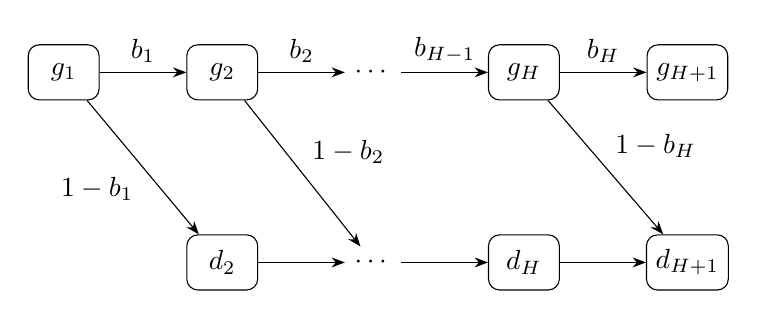
\begin{tikzpicture}[>=Stealth,node distance=11mm,
  state/.style={draw,rounded corners,minimum width=9mm,minimum height=7mm}]
 \node[state] (g1) {$g_1$};
 \node[state,right=of g1] (g2) {$g_2$};
 \node[right=of g2] (dots) {$\cdots$};
 \node[state,right=of dots] (gh) {$g_H$};
 \node[state,right=of gh] (gt) {$g_{H+1}$};
 \node[state,below=17mm of g2] (d2) {$d_2$};
 \node (ddots) at (dots |- d2) {$\cdots$};
 \node[state] (dh) at (gh |- d2) {$d_H$};
 \node[state] (dt) at (gt |- d2) {$d_{H+1}$};
 \draw[->] (g1)--node[above] {$b_1$}(g2);
 \draw[->] (g2)--node[above] {$b_2$}(dots);
 \draw[->] (dots)--node[above] {$b_{H-1}$}(gh);
 \draw[->] (gh)--node[above] {$b_H$}(gt);
 \draw[->] (g1)--node[below left] {$1-b_1$}(d2);
 \draw[->] (g2)--node[above right] {$1-b_2$}(ddots);
 \draw[->] (gh)--node[above right] {$1-b_H$}(dt);
 \draw[->] (d2)--(ddots);
 \draw[->] (ddots)--(dh);
 \draw[->] (dh)--(dt);
\end{tikzpicture}
\end{center}
The diagram shows some of the transitions. Every transition along the lower
row permits either action; terminal self-loops are omitted.
Reaching $g_h$ means that the first $h-1$ actions matched
$b_1,\ldots,b_{h-1}$. After the first mismatch, the process remains among
the failed states for the rest of the episode. The transition kernel is
time-homogeneous because the layer is part of the state.
The examples below specify the teacher and what the learner knows about
$b$. Rewards will be introduced in \cref{sec:rl}.

\section{Review: how errors can compound}
\label{sec:compounding}

Lecture 4, Sections 4.3.2--4.3.3, compared sequence generators at a fixed
forward KL divergence from the data law. In its binary model of language
generation, a one represented an incorrect step. The \emph{error count}
$c_{\mathrm{cnt}}$ counted incorrect steps, while the \emph{terminal cost}
$c_{\mathrm{fin}}$ recorded whether the final answer was wrong.
For a sequence law $Q$ and the all-zero data sequence, fixing sequence KL
at $\kappa\ge0$ fixes only the probability of generating that sequence:
\[
 \KL(\delta_{0^H}\Vert Q)=\kappa
 \quad\Longleftrightarrow\quad Q(0^H)=e^{-\kappa}.
\]
The costs also depend on what happens after a first error: the generator
may recover or continue producing incorrect steps. Lecture 4's examples
showed that these behaviors can have the same KL divergence.

In the policy/environment framework, an early wrong action changes the
states encountered later and can cause costs at many subsequent steps.
We call this accumulation of an error's effects \emph{compounding error}.
We now express Lecture 4's persistent-error calculation from Exercises 9--10
in the layered environment of \cref{ex:layered}. More decisions create
more opportunities for a first error; persistence determines how many
later steps that error affects.

The following example asks what a one-step imitation-error guarantee alone
can imply. We specify a candidate policy with error probability $p$ at
each teacher-visited state, then calculate its costs over a complete episode.
A performance bound based only on that local accuracy must cover this
candidate policy.

\begin{example}[Persistent errors in the layered environment]
\label{ex:first-error}
Use \cref{ex:layered} with $b=0^H$. The teacher always chooses action $0$,
so its state at stage $h$ is $g_h$.

Fix $p\in[0,1]$. At each $g_h$, the candidate policy $\pi$ chooses action $1$
with probability $p$, using fresh randomness at each decision. At each $d_h$,
let it choose action $0$; failure persists even though that action agrees
with the teacher. The learner's error on teacher-visited states is $p$.

For a trajectory $T$, define the error count and terminal cost by
\[
 c_{\mathrm{cnt}}(T)=\sum_{h=1}^H\I\{S_{h+1}=d_{h+1}\},\qquad
 c_{\mathrm{fin}}(T)=\I\{S_{H+1}=d_{H+1}\}.
\]
The error count records erroneous post-decision states, and the terminal
cost records whether the final result is wrong. The teacher has zero cost
under both assessments.

All probabilities below concern a trajectory generated by the learner. Let
$F=\min\{h:A_h=1\}$, with $F=\infty$ if no such step occurs.
Since $\{S_{h+1}=d_{h+1}\}=\{F\le h\}$, the terminal cost satisfies
\begin{equation}
 v_{c_{\mathrm{fin}}}(\pi)=\P(F\le H)=1-(1-p)^H\le Hp.
 \label{eq:first-error}
\end{equation}
For the error count, which is a cumulative cost,
\begin{equation}
 v_{c_{\mathrm{cnt}}}(\pi)=\sum_{h=1}^H\P(F\le h)
          =\sum_{h=1}^H\bigl(1-(1-p)^h\bigr).
 \label{eq:cumulative-error}
\end{equation}
If $Hp\le1$, these quantities satisfy
\begin{equation}
 \frac{Hp}{2}\le v_{c_{\mathrm{fin}}}(\pi)\le Hp,\qquad
 \frac{pH(H+1)}4\le v_{c_{\mathrm{cnt}}}(\pi)\le\frac{pH(H+1)}2.
 \label{eq:compounding-bounds}
\end{equation}
\end{example}

To verify the lower bounds, use $\log(1-p)\le-p$ to obtain
$(1-p)^h=\exp(h\log(1-p))\le e^{-hp}$ for $p<1$; the bound also holds
at $p=1$. Then $e^u\le1+u+u^2/2$ for $u\le0$ gives, when $hp\le1$,
\[
 1-(1-p)^h
 \ge1-e^{-hp}
 \ge hp-\frac{h^2p^2}{2}
 \ge\frac{hp}{2}.
\]
The upper bounds follow from the union bound. Thus expected terminal cost
is of order $Hp$, while expected error count is of order $H^2p$ in the
stated range. The terminal cost counts an episode once if it ends in error.
The error count counts every erroneous result along the trajectory, so an early
error can contribute at every remaining step. This persistence and the
unnormalized sum account for the second factor of $H$.

\begin{remark}[Distribution shift]
\label{rem:compounding}
The \emph{distribution shift} here is the difference between the teacher's
and the learner's state distributions at the same stage. In
\cref{ex:first-error}, the teacher always visits $g_h$, whereas a learner
that has made an error visits $d_h$. A bound based only on local
prediction error under teacher states may therefore incur horizon factors
when converted to a bound on complete episodes.
\end{remark}

\Cref{ex:first-error} shows that a guarantee based only on local error must
allow these horizon factors. A learner could achieve $p=0$ in this simple problem.
To determine sample complexity, we must also examine what the training
objective controls and how its accuracy depends on the dataset.
The example uses a deterministic teacher only to isolate the mechanism;
the likelihood analysis that follows allows arbitrary stochastic teachers.

\section{Review: log loss as a trajectory likelihood}
\label{sec:likelihood}

The sequence-likelihood identity and KL chain rule below are the results
from Lecture 4, Section 4.1. Here we write them for a policy acting in a
common environment. Log-loss behavior cloning evaluates conditional
predictions at the teacher's
observed states. Its statistical meaning comes from the joint law of the
observations: those states and actions form complete trajectories.
We first identify the likelihood objective and then distinguish its population
meaning from a finite-sample guarantee.

\subsection{The empirical objective}

Let $\Pi$ be a class of policies. The per-trajectory empirical log loss is
\begin{equation}
 L_n(\pi)
   =\frac1n\sum_{i=1}^n\sum_{h=1}^H
       -\log\pi_h(A_h^i\mid S_h^i).
 \label{eq:bc}
\end{equation}
A zero probability assigned to an observed action gives infinite loss.
Log-loss behavior cloning minimizes \cref{eq:bc}; dividing by $H$ gives
the corresponding per-token or per-action average and leaves exact
minimizers unchanged. In language modeling, this is the usual teacher-forced
supervised fine-tuning objective.

The connection to complete trajectories follows directly from
\cref{eq:trajectory-law}. On every trajectory with positive teacher
probability,
\begin{equation}
 -\log P^\pi(\tau)=
 -\log\mu(s_1)-\sum_{h=1}^H\log P(s_{h+1}\mid s_h,a_h)
 -\sum_{h=1}^H\log\pi_h(a_h\mid s_h).
 \label{eq:likelihood-factors}
\end{equation}
Only the last sum depends on the policy. Minimizing $L_n$ is
therefore maximum likelihood over the trajectory models
$\{P^\pi:\pi\in\Pi\}$. The learner need not know the environment factors
to perform this minimization.

Teacher forcing evaluates each factor at the recorded prefix. The same
factors define the learner's joint distribution when it generates a fresh
trajectory. This equality between the training likelihood and the generative
model is the reason that a trajectory-level analysis is available.

\subsection{The population identity and its limitation}

Lecture 4, Section 4.1, decomposed population log loss into data entropy
and forward KL. The analogous identity here compares the learner's
population loss with the teacher's population loss.
Let $T$ have the teacher's law, write $P=P^{\pi^{\rm E}}$, and set
$L(\pi)=\E[\sum_{h=1}^H-\log\pi_h(A_h\mid S_h)]$.
For probability masses $P,Q$, use
$\KL(P\Vert Q)=\sum_{\tau:P(\tau)>0}P(\tau)\log(P(\tau)/Q(\tau))$,
with value infinity when $Q$ vanishes on a point of positive $P$ mass.

\begin{proposition}[Trajectory KL identity]
\label{prop:kl}
In the common environment of \cref{sec:setup}, every policy $\pi$ satisfies
\begin{equation}
 L(\pi)-L(\pi^{\rm E})
 =\KL(P^{\pi^{\rm E}}\Vert P^\pi)
 =\sum_{h=1}^H
   \E\!\left[\KL\bigl(\pi_h^{\rm E}(\cdot\mid S_h)
                 \Vert\pi_h(\cdot\mid S_h)\bigr)\right].
 \label{eq:kl-chain}
\end{equation}
\end{proposition}

\begin{proof}
The common initial-state and transition factors cancel in the likelihood
ratio, so
\[
 \log\frac{P^{\pi^{\rm E}}(T)}{P^\pi(T)}
 =\sum_{h=1}^H
   \log\frac{\pi_h^{\rm E}(A_h\mid S_h)}{\pi_h(A_h\mid S_h)}.
\]
Take expectations under the teacher law. Conditional on $S_h$, the action
$A_h$ has law $\pi_h^{\rm E}(\cdot\mid S_h)$, which gives the last expression
in \cref{eq:kl-chain}. The difference of population log losses gives the
first expression. If the learner assigns zero probability to a
teacher-supported action at a teacher-visited state, both sides are infinite.
\end{proof}

The teacher's population loss is the sum of its conditional action
entropies, averaged over the states it visits:
\[
 L(\pi^{\rm E})
 =\sum_{h=1}^H\E\!\left[
   -\sum_{a\in\cA}\pi_h^{\rm E}(a\mid S_h)
                    \log\pi_h^{\rm E}(a\mid S_h)\right],
 \qquad 0\log0:=0.
\]
By \cref{prop:kl}, $L(\pi)\ge L(\pi^{\rm E})$ for every policy.
Thus $L(\pi^{\rm E})$ is the minimum possible population loss; it is
positive whenever the teacher randomizes at a state--stage pair reached
with positive probability. The \emph{excess log loss}
$L(\pi)-L(\pi^{\rm E})$ is the loss above this minimum. By the same
identity, this excess equals the trajectory KL divergence and is zero
exactly when $P^\pi=P^{\pi^{\rm E}}$. The entropy term is independent
of the learner, so minimizing $L(\pi)$ also minimizes the excess.

The chain rule also shows how local excess losses accumulate.
If the average per-stage excess loss is at most
$\varepsilon$, then
\begin{equation}
 \KL(P^{\pi^{\rm E}}\Vert P^\pi)\le H\varepsilon,
 \qquad
 \TV(P^{\pi^{\rm E}},P^\pi)\le\sqrt{H\varepsilon/2},
 \label{eq:population-pin}
\end{equation}
where the second inequality is Pinsker's inequality. To certify a fixed
total-variation accuracy through this bound, the per-stage excess loss must
decrease proportionally to $1/H$.

We can now express the costs in \cref{ex:first-error} in terms of excess
log loss. The teacher always takes action $0$ at $g_h$, and the candidate
policy assigns that action probability $1-p$. For $p<1$,
\[
 L(\pi^{\rm E})=0,\qquad
 \kappa:=L(\pi)-L(\pi^{\rm E})=-H\log(1-p).
\]
Substituting $1-p=e^{-\kappa/H}$ in the cost formulas gives
\[
 v_{c_{\mathrm{fin}}}(\pi)=1-e^{-\kappa},\qquad
 v_{c_{\mathrm{cnt}}}(\pi)=\sum_{h=1}^H(1-e^{-h\kappa/H}).
\]
Thus a fixed whole-trajectory excess log loss fixes terminal error
independently of $H$. A fixed positive local error probability $p$ instead makes
that excess loss grow linearly with $H$.

\subsection{What changes when the data are reorganized?}

Shuffling all recorded state--action pairs before optimization leaves
\cref{eq:bc} unchanged, provided each pair retains its state or full prefix
and its stage when the policy is stage-dependent. Shuffling also leaves
the dependence among the observations unchanged. The learner is still
minimizing the likelihood of the original independent episodes.

A different experiment samples independent pairs separately at every stage,
with the stage-$h$ pair distributed as $(S_h,A_h)$ under the teacher.
The expected sum of conditional losses is still $L(\pi)$, so
\cref{prop:kl} remains the population identity. The finite-sample data law,
however, is now a product of stage marginals rather than a product of
complete-trajectory laws. A likelihood-ratio proof for complete episodes
cannot simply be applied by stitching these independent pairs together.
The next theorem uses the actual episode sampling model.\endnote{With known
dynamics, independently sampled states can themselves carry information
about the teacher. A conditional action likelihood ignores that part of the
snapshot likelihood. In \cref{ex:repeated-bit}, a later independently
sampled state reveals the first action and hence carries information about
the parameter $p$. Within a recorded full trajectory, that state merely repeats
information already present in the first action. The two sampling models
must be distinguished before claiming an information advantage.}

\section{Review: a finite-sample guarantee for stochastic teachers}
\label{sec:finite}

The finite-sample result in this section is the likelihood guarantee from
Lecture 4, supplementary Section 4.4.4; its proof appeared in Appendix 4.D.1.
We give the argument here in trajectory notation to answer what empirical
log-loss minimization guarantees from $n$ independent demonstrations.
A direct likelihood argument controls a
distance between complete trajectory laws without first estimating a
one-step error and multiplying by the horizon.

\subsection{Likelihood controls Hellinger distance}

We will use Hellinger distance to state the likelihood guarantee. A Bernoulli
calculation first explains what accuracy in this distance means statistically.
The likelihood proof then supplies the reason for choosing Hellinger distance:
an exact identity converts a likelihood comparison into a distance bound.
Define the squared \emph{Hellinger distance} and its square root by
\begin{equation}
 h^2(P,Q)=\sum_{\tau\in\cT}
       \bigl(\sqrt{P(\tau)}-\sqrt{Q(\tau)}\bigr)^2,\qquad
 h(P,Q)=\sqrt{h^2(P,Q)}.
 \label{eq:hellinger}
\end{equation}
Writing $\sqrt P=(\sqrt{P(\tau)})_{\tau\in\cT}$, we have
\[
 \|\sqrt P\|_2^2=\sum_\tau P(\tau)=1,\qquad
 \langle\sqrt P,\sqrt Q\rangle=1-\frac{h^2(P,Q)}2.
\]
Thus Hellinger distance is the Euclidean distance between square-root
probability vectors. These vectors have norm one and nonnegative
coordinates, so $0\le h^2\le2$. The inner-product identity will be useful
in the likelihood proof.

\paragraph{A Bernoulli calculation.}
Suppose $X_1,\ldots,X_n$ are independent $\operatorname{Bernoulli}(p)$
observations, with $p\in(0,1)$. The empirical frequency
$\widehat p=n^{-1}\sum_{i=1}^nX_i$ estimates $p$, and
\[
 \E[\widehat p]=p,\qquad
 \operatorname{Var}(\widehat p)=\frac{p(1-p)}n,\qquad
 \sigma_n=\sqrt{\frac{p(1-p)}n}.
\]
The standard deviation $\sigma_n$ describes how much the empirical frequency
varies across independent datasets. Measuring a probability error in units
of $\sigma_n$ compares that error with the sampling variability. The next
proposition shows that squared Hellinger distance makes the same comparison
locally, after multiplication by $n$.

\Needspace{12\baselineskip}
\begin{proposition}[Hellinger distance in standard-deviation units]
\label{prop:hellinger-bernoulli}
Fix $p\in(0,1)$ and write $P=\operatorname{Bernoulli}(p)$,
$Q_\varepsilon=\operatorname{Bernoulli}(p+\varepsilon)$, where
$p+\varepsilon\in(0,1)$. With $\sigma_n^2=p(1-p)/n$, as
$\varepsilon\to0$,
\begin{equation}
 h^2(P,Q_\varepsilon)\sim\frac{\varepsilon^2}{4p(1-p)},\qquad
 n h^2(P,Q_\varepsilon)\sim\frac14\left(\frac{\varepsilon}{\sigma_n}\right)^2.
 \label{eq:hellinger-bernoulli}
\end{equation}
Here $\sim$ means that the ratio of the two sides tends to one.
In particular, for any fixed $c\in\R$, setting
$\varepsilon_n=c\sigma_n$ gives
\begin{equation}
 \lim_{n\to\infty}n h^2(P,Q_{\varepsilon_n})=\frac{c^2}{4}.
 \label{eq:hellinger-sampling-scale}
\end{equation}
\end{proposition}

\begin{proof}
Using $(\sqrt a-\sqrt b)^2=(a-b)^2/(\sqrt a+\sqrt b)^2$ for $a,b>0$,
\[
 h^2(P,Q_\varepsilon)
 =\frac{\varepsilon^2}{(\sqrt{p+\varepsilon}+\sqrt p)^2}
  +\frac{\varepsilon^2}{(\sqrt{1-p-\varepsilon}+\sqrt{1-p})^2}.
\]
As $\varepsilon\to0$, the two denominators approach $4p$ and $4(1-p)$.
Their reciprocal limits sum to $1/[4p(1-p)]$, proving the first relation
in \cref{eq:hellinger-bernoulli}. Multiplying by $n$ and substituting
$\sigma_n^2=p(1-p)/n$ proves the second. For $c\ne0$, substitute
$\varepsilon_n=c\sigma_n\to0$ to obtain
\cref{eq:hellinger-sampling-scale}; for $c=0$, the distance is zero.
Since $p\in(0,1)$, $p+\varepsilon_n$ lies in $(0,1)$ for all sufficiently
large $n$.
\end{proof}

An error of a fixed nonzero number of standard deviations therefore corresponds
to squared Hellinger distance of order $1/n$. The proposition gives us
a reference scale for a learning guarantee: in the Bernoulli example,
a bound of order $1/n$ on squared Hellinger error corresponds locally to
a bounded error in standard-deviation units. Other distances have related
local interpretations; the likelihood proof will use a further property
of Hellinger distance.\endnote{\emph{Connection to Fisher information.}
Consider positive probability masses $p_\theta(x)$ on a finite set,
twice continuously differentiable in $\theta$ on an open subset of $\R^d$.
For $X\sim P_\theta$, define the \emph{score}
$s_\theta(x)=\nabla_\theta\log p_\theta(x)$ and the
\emph{Fisher information matrix}
$I(\theta)=\E[s_\theta(X)s_\theta(X)^\top]$.
Since $\nabla_\theta\sqrt{p_\theta(x)}
=\tfrac12\sqrt{p_\theta(x)}s_\theta(x)$, expansion and summation give
\[
 h^2(P_\theta,P_{\theta+u})
 =\tfrac14u^\top I(\theta)u+o(\|u\|^2).
\]
The remainder divided by $\|u\|^2$ tends to zero as $u\to0$.
The same assumptions give
$\KL(P_\theta\Vert P_{\theta+u})
=\tfrac12u^\top I(\theta)u+o(\|u\|^2)$.
Thus Hellinger distance and KL have the same local quadratic form up to a
constant; that local geometry does not uniquely select Hellinger distance.
For the Bernoulli laws in \cref{prop:hellinger-bernoulli},
$\TV(P,Q_\varepsilon)=|\varepsilon|$, so
$\TV^2(P,Q_{c\sigma_n})=c^2p(1-p)/n$.
Squared total variation also has order $1/n$ at the sampling scale for
fixed $p$ and nonzero $c$, with a coefficient depending on $p$.
The $n^{-1/2}$ parameter-error scale of regular asymptotic estimation
corresponds to a squared Hellinger distance of order $1/n$ in directions
with positive Fisher information. More general asymptotic theory uses
differentiability of square-root densities in squared-integral norm;
the bibliographical notes give a reference.}\label{en:fisher}

\paragraph{A distance for the likelihood guarantee.}
The inner-product identity above gives an exact relation to likelihood.
For arbitrary trajectory laws $P,Q$ and an observation $T\sim P$,
\[
 \E\!\left[\sqrt{\frac{Q(T)}{P(T)}}\right]
 =\langle\sqrt P,\sqrt Q\rangle
 =1-\frac{h^2(P,Q)}2.
\]
The expectation of the square-root likelihood ratio therefore decreases
with squared Hellinger distance. In the proof below, independence and
Markov's inequality turn this identity into a bound of
$\exp(-nh^2(P,Q)/2)$ on the probability that a fixed candidate $Q$ fits
the sample at least as well as the teacher $P$.
A union bound over a finite class containing the teacher then gives, for
exact optimization,
$h^2(P^{\pi^{\rm E}},P^{\widehat\pi})\le2\log(|\Pi|/\delta)/n$
with probability at least $1-\delta$.
The resulting guarantee has the $1/n$ scale interpreted by
\cref{prop:hellinger-bernoulli}, with a logarithmic factor for the class
size and confidence.

Hellinger distance also controls total variation:
\begin{equation}
 \TV(P,Q)
 = \frac12 \|P-Q\|_1
 \le\frac12
 \sqrt{\sum_\tau(\sqrt P-\sqrt Q)^2
              \sum_\tau(\sqrt P+\sqrt Q)^2}
 \le h(P,Q).
 \label{eq:tv-hellinger}
\end{equation}
The first inequality is Cauchy--Schwarz, after factoring $P-Q$.
We assume the policy class contains the teacher, a condition called
\emph{realizability}.

\Needspace{15\baselineskip}
\begin{theorem}[Finite-class log-loss behavior cloning]
\label{thm:bc}
Let $\Pi$ be a finite policy class containing the stochastic teacher
$\pi^{\rm E}$. Let $T^1,\ldots,T^n$ be independent trajectories with law
$P^{\pi^{\rm E}}$, where $n\ge1$. Fix $\eta\ge0$, and suppose the learned
policy $\widehat\pi\in\Pi$ satisfies
\begin{equation}
 \frac{L_n(\widehat\pi)}{H}
 \le \min_{\pi\in\Pi}\frac{L_n(\pi)}{H}+\eta.
 \label{eq:approx-mle}
\end{equation}
For every $\delta\in(0,1)$, with probability at least $1-\delta$,
\begin{equation}
 h^2(P^{\pi^{\rm E}},P^{\widehat\pi})\le b,
 \qquad b=\frac{2\log(|\Pi|/\delta)}n+H\eta.
 \label{eq:bc-bound}
\end{equation}
In particular, on the same event,
$\TV(P^{\pi^{\rm E}},P^{\widehat\pi})\le\sqrt b$.
\end{theorem}

\begin{proof}
Write $P=P^{\pi^{\rm E}}$ and fix a candidate trajectory law $Q=P^\pi$.
The random variables in this proof are the independent teacher trajectories.
The teacher belongs to the policy class, so a selected policy must have
empirical loss at most $H\eta$ above the teacher's. We will show that each
distant candidate is unlikely to satisfy this comparison, then account
for all the candidates by a union bound.

The \emph{likelihood ratio} compares the probabilities that $Q$ and $P$
assign to the observed sample:
\[
 R_Q=\prod_{i=1}^n\frac{Q(T^i)}{P(T^i)}
 =\exp\!\left(n[L_n(\pi^{\rm E})-L_n(\pi)]\right).
\]
The denominators are positive almost surely, and the equality uses
cancellation of the common environment factors. Hence the empirical-loss
comparison is exactly the event $R_Q\ge e^{-nH\eta}$.

To bound that event, we may apply Markov's inequality to any positive power
of $R_Q$: for $a>0$ and $\alpha>0$,
\[
 \P(R_Q\ge a)=\P(R_Q^\alpha\ge a^\alpha)
 \le a^{-\alpha}\E[R_Q^\alpha].
\]
Which power gives an informative expectation? The choice $\alpha=1$ gives
$\E[R_Q]=(\sum_{\tau:P(\tau)>0}Q(\tau))^n$, which equals one whenever
$Q$ assigns no mass outside the support of $P$. In that case, the expectation
does not distinguish a nearby candidate from a distant one.
For $0<\alpha<1$, independence instead gives
\[
 \E[R_Q^\alpha]
 =\left(\sum_{\tau\in\cT}P(\tau)^{1-\alpha}Q(\tau)^\alpha\right)^n.
\]
Choosing $\alpha=1/2$ makes the sum symmetric in $P$ and $Q$ and relates it
directly to squared Hellinger distance. Put
\[
 Z_Q=\sqrt{R_Q}=\prod_{i=1}^n\sqrt{\frac{Q(T^i)}{P(T^i)}}.
\]
Then
\begin{equation}
 \E[Z_Q]
 =\left(\sum_{\tau\in\cT}\sqrt{P(\tau)Q(\tau)}\right)^n
 =\bigl(1-h^2(P,Q)/2\bigr)^n
 \le \exp\bigl(-nh^2(P,Q)/2\bigr).
 \label{eq:affinity}
\end{equation}
The expectation now decreases with the distance of the candidate from the
teacher. Taking $a=e^{-nH\eta}$ in the Markov bound therefore gives
\begin{equation}
 \P\{L_n(\pi)\le L_n(\pi^{\rm E})+H\eta\}
 \le \exp\!\left(-\frac n2[h^2(P,Q)-H\eta]\right).
 \label{eq:bad-likelihood}
\end{equation}
For each candidate with $h^2(P,Q)>b$, the right-hand side is at most
$\delta/|\Pi|$. A union bound shows that, with probability at least
$1-\delta$, no such candidate has empirical loss within $H\eta$ of the
teacher's empirical loss. Since $\pi^{\rm E}\in\Pi$,
\cref{eq:approx-mle} puts $\widehat\pi$ within this loss tolerance.
Hence its squared Hellinger distance is at most $b$.
\end{proof}

The proof rules out distant candidates by comparing their likelihoods with
the teacher's likelihood. The factor $n$ in the exponential bound comes
from independent demonstrations; the logarithm of the class size comes
from requiring the comparison to hold for every candidate that training
could select.
The proof treats one episode as one independent observation, with all its
conditional action probabilities included in the likelihood ratio. No
independence within an episode was used. The same proof applies to stochastic
teachers because it compares probability laws directly.

The theorem controls Hellinger distance, not forward KL. Empirical maximum
likelihood can assign zero probability to an outcome that happened not to
appear in the sample, making $\KL(P^{\pi^{\rm E}}\Vert P^{\widehat\pi})$
infinite. \Cref{ex:l18-likelihood-support} gives a two-model example.
The population KL identity and the finite-sample Hellinger theorem serve
different purposes.

\subsection{From distribution accuracy to performance}

To interpret the statistical guarantee, we translate it to the cost in
\cref{eq:cost}. Total variation gives
$|\Delta_c(\widehat\pi)|\le C_{\max}\sqrt b$.
The variance-sensitive inequality from Lecture 4, Proposition 4.C.1,
can be sharper when the teacher's cost varies little across its trajectories.
We recall the inequality and its proof.

\Needspace{10\baselineskip}
\begin{proposition}[Cost transfer]
\label{prop:cost-transfer}
Let $P,Q$ be probability masses on $\cT$, and let
$c:\cT\to[0,C_{\max}]$. Define
$\bar c=\sum_\tau P(\tau)c(\tau)$ and
$\sigma_P^2(c)=\sum_\tau P(\tau)(c(\tau)-\bar c)^2$.
Then
\begin{equation}
 \left|\sum_\tau [P(\tau)-Q(\tau)]c(\tau)\right|
 \le 2\sigma_P(c)h(P,Q)+C_{\max}h^2(P,Q).
 \label{eq:cost-transfer}
\end{equation}
\end{proposition}

\begin{proof}
Regard $P,Q,c$ as vectors indexed by $\cT$, with products and squares
taken coordinatewise, and let $\mathbf1$ be the all-ones vector.
Set $u=\sqrt P-\sqrt Q$. Then
\[
 P-Q=2\sqrt P\,u-u^2,\qquad
 \langle P-Q,\mathbf1\rangle=0,\qquad
 \|u\|_2^2=\|u^2\|_1=h^2(P,Q).
\]
The variance definition and $0\le\bar c\le C_{\max}$ give
\[
 \|\sqrt P(c-\bar c\mathbf1)\|_2=\sigma_P(c),\qquad
 \|c-\bar c\mathbf1\|_\infty\le C_{\max}.
\]
Cauchy--Schwarz and the $\ell^1$--$\ell^\infty$ inequality now give
\[
\begin{aligned}
 |\langle Q-P,c\rangle|
 &=|\langle P-Q,c-\bar c\mathbf1\rangle|\\
 &=\bigl|2\langle u,\sqrt P(c-\bar c\mathbf1)\rangle
          -\langle u^2,c-\bar c\mathbf1\rangle\bigr|\\
 &\le2\|u\|_2\|\sqrt P(c-\bar c\mathbf1)\|_2
       +\|u^2\|_1\|c-\bar c\mathbf1\|_\infty\\
 &\le2\sigma_P(c)h(P,Q)+C_{\max}h^2(P,Q).
\end{aligned}
\]
\end{proof}

\begin{corollary}[Performance of the cloned policy]
\label{cor:performance}
On the event in \cref{thm:bc}, every cost
$c:\cT\to[0,C_{\max}]$ satisfies
\begin{equation}
 |\Delta_c(\widehat\pi)|
 \le 2\sigma_{P^{\pi^{\rm E}}}(c)\sqrt b+C_{\max}b.
 \label{eq:performance}
\end{equation}
If the teacher has zero cost with probability one, then
$v_c(\widehat\pi)\le C_{\max}b$.
\end{corollary}

The last conclusion permits a stochastic teacher: the teacher may randomize
among many zero-cost trajectories. The improved rate comes from zero cost
variance, not from determinism of its actions. For a general stochastic
teacher and a general cost, the square-root term remains.
All these evaluations use the same learned policy; the training algorithm
never receives the cost function.

\subsection{In what sense is there no extra horizon factor?}

For exact empirical minimization, $b=2\log(|\Pi|/\delta)/n$. With the
policy-class size, the number of independent demonstrations, and the cost
range fixed, the theorem has no explicit horizon factor. A separate
conversion from teacher-state error to learner-state error is unnecessary:
the estimated object is already the complete trajectory law.

Several quantities may change when the horizon changes. A class of
unrelated stage-wise policies can become larger with $H$. An unnormalized
cumulative cost has range $H$. A fixed number of sampled teacher actions
buys fewer complete trajectories when those trajectories are longer.
Finally, a per-action optimization tolerance $\eta$ contributes $H\eta$;
keeping that contribution below the statistical term requires
$\eta\le 2\log(|\Pi|/\delta)/(nH)$. The optimization issue is the same
loss-normalization issue encountered in Lecture 4.

Thus log-loss behavior cloning can avoid an \emph{additional statistical
penalty} attributed to compounding error under the theorem's assumptions.
It cannot make a fixed local prediction discrepancy harmless at arbitrarily
long horizons. \Cref{eq:population-pin} and \cref{thm:bc} are consistent:
the first starts from a specified local population error; the second derives
trajectory accuracy from a complete-trajectory training experiment.

\section{How much information is in a demonstration?}
\label{sec:information}

Lecture 6, Section 6.4, showed why exact copies do not provide independent
observations; Lecture 4, Section 4.4.1, discussed the information available
for shared parameters. We apply those principles to a different question:
how many informative observations does a budget of teacher actions buy?
The sample unit in \cref{thm:bc} is an independent trajectory. A long
trajectory may contain many informative teacher decisions, or it may repeat
the consequence of one decision. A stochastic example will make this
distinction exact and provide a setting in which interaction helps.

\Needspace{14\baselineskip}
\begin{example}[One random decision, repeated for the whole episode]
\label{ex:repeated-bit}
Use the same layered environment, now with $b=0^H$ known to the learner.
The unknown parameter is $p\in[1/4,3/4]$. At $g_1$, the teacher draws
its first action $B\sim\operatorname{Bernoulli}(p)$. At later stages,
it chooses $0$ at $g_h$ and $1$ at $d_h$:
\[
 \pi_h^{\rm E}(1\mid g_h)=0,\qquad
 \pi_h^{\rm E}(1\mid d_h)=1,\qquad 2\le h\le H.
\]
All other state--stage action distributions are fixed, known, and
independent of $p$. A first action $0$ therefore gives $0^H$, whereas
a first action $1$ gives $1^H$. The learner knows the continuation rule
and only needs to estimate $p$. The teacher's action sequence has law
\begin{equation}
 P_p(1^H)=p,\qquad P_p(0^H)=1-p.
 \label{eq:repeated-bit}
\end{equation}
The deterministic states add no further information. A learner using
the same continuation rule and first-action parameter $q$ has action law
$P_q$. The complete trajectory is determined by its actions, so the
following distances also equal those between the complete trajectory laws:
\begin{equation}
 \TV(P_p,P_q)=|p-q|,\qquad
 \KL(P_p\Vert P_q)
 =p\log\frac pq+(1-p)\log\frac{1-p}{1-q}.
 \label{eq:repeated-distances}
\end{equation}
\end{example}

Each trajectory reveals one Bernoulli draw. The later actions confirm a
known rule and reveal nothing further about $p$. For $n$ independent
trajectories, write their first actions as $B_1,\ldots,B_n$. Maximum
likelihood estimates $p$ by the sample mean, clipped to $[1/4,3/4]$:
\[
 \widehat p=\min\{3/4,\max\{1/4,\overline B_n\}\},
 \qquad \overline B_n=\frac1n\sum_{i=1}^n B_i.
\]
Clipping cannot increase the distance from $p$. Independence gives
\begin{equation}
 \E[|\widehat p-p|]
 \le \sqrt{\E[(\overline B_n-p)^2]}
 =\sqrt{\frac{p(1-p)}n}\le\frac1{2\sqrt n}.
 \label{eq:bernoulli-upper}
\end{equation}
Expectations here concern the independent training bits at the fixed
parameter $p$. This continuous family is analyzed directly; we are not
substituting an infinite $\Pi$ into the finite-class theorem.

The $n^{-1/2}$ rate cannot be improved uniformly over this family.
\Cref{app:bernoulli} proves that, for any estimator $\widetilde p$ based
on $n$ such observations, including a randomized estimator,
\begin{equation}
 \sup_{p\in[1/4,3/4]}\E[|\widetilde p-p|]\ge\frac1{32\sqrt n}.
 \label{eq:bernoulli-lower}
\end{equation}
The expectation includes any estimator randomness independent of the data.
Together with \cref{eq:repeated-distances}, this gives matching orders for
the worst-case expected trajectory total-variation error.

The absence of an $H$ factor at fixed $n$ is now easy to interpret.
Extending a demonstration by more repetitions gives no extra information,
but it also creates no new unknown parameter. If the budget instead counts
teacher actions, $m=nH$ actions buy only $n=m/H$ independent bits, and
the worst-case error has order
\begin{equation}
 \sqrt{\frac Hm}.
 \label{eq:offline-budget}
\end{equation}
The horizon dependence in \cref{eq:offline-budget} is a data-acquisition
cost, not error propagation during deployment.

Dependence does not imply that every trajectory contains only one useful
observation. If the teacher instead draws a fresh
$\operatorname{Bernoulli}(p)$ action independently at every stage, $n$
trajectories contain $nH$ independent draws. The variance of their overall
sample mean is $p(1-p)/(nH)$. As in Lecture 6, the information available
for a particular parameter depends on the joint data law, not just on the
number of rows in a dataset.

\section{What interaction can buy in imitation learning}
\label{sec:interaction}

The new question is whether choosing which teacher decisions to observe
improves accuracy at a fixed data-acquisition cost.
A comparison with offline learning is meaningful only after we
specify the available queries and their cost. We use the repeated-bit family
to give an exact separation without rewards or a deterministic teacher.

\subsection{A teacher-action budget comparison}

Suppose a \emph{teacher-action query} supplies a state and stage and returns a
fresh action sampled from the teacher's conditional distribution there.
The learner may restart at the initial state. Each returned teacher action
costs one unit; a complete length-$H$ demonstration costs $H$ units.
The oracle returns a sampled action, not the teacher's probabilities.
In \cref{ex:repeated-bit}, querying the initial state repeatedly therefore
returns independent $\operatorname{Bernoulli}(p)$ draws.

\begin{proposition}[Selective queries save a factor of the horizon]
\label{prop:interaction}
In the known repeated-bit family, let the teacher-action budget be
$m=nH$, with positive integers $n,H$. If data must consist of complete
demonstrations, the smallest worst-case expected trajectory
total-variation error is of order $\sqrt{H/m}$.
If the learner may query the initial teacher decision separately, the
smallest worst-case expected error is of order $1/\sqrt m$.
\end{proposition}

\begin{proof}
Complete demonstrations provide exactly $n=m/H$ independent Bernoulli
draws. The upper bound \cref{eq:bernoulli-upper} and lower bound
\cref{eq:bernoulli-lower} apply.
For the interactive upper bound, query the initial state $m$ times,
estimate $p$ by the clipped sample mean, and use the known repetition rule
after the first decision. The same bounds now apply with $m$ draws.
For the interactive lower bound, every query except $(1,g_1)$ has a known
response law independent of $p$. Any transcript of at most $m$ queries can be
simulated from $m$ independent Bernoulli draws and independent learner
randomness. Hence \cref{eq:bernoulli-lower}, with $n=m$, also lower-bounds
the best interactive estimator.
\end{proof}

For a small target expected error $\varepsilon$, complete demonstrations
require order $H/\varepsilon^2$ teacher actions, whereas selected queries
require order $1/\varepsilon^2$. The advantage is a factor $H$ in
teacher-action sample complexity, or a factor $\sqrt H$ in accuracy at
a fixed budget. Both protocols observe samples from the same stochastic
teacher.

The source of the improvement is known in this example: only the first
decision depends on the unknown parameter. The query schedule is
nonadaptive: query the initial state every time. The proposition establishes the
potential benefit of allocating queries to informative decisions. It does
not provide an algorithm that discovers where those decisions occur in an
arbitrary policy class. If obtaining an initial-state response has an
additional setup cost, that cost must be included before drawing a
computational comparison.

There is also a simple family with no such information advantage.
For the independent-bit teacher described at the end of
\cref{sec:information}, every queried action is a fresh
$\operatorname{Bernoulli}(p)$ draw, regardless of its stage or state.
With $m$ returned actions, both passive collection and adaptive queries
provide exactly the same $m$ Bernoulli observations about $p$. Adaptively
choosing their contexts cannot improve estimation by creating information
that the responses do not contain.

\subsection{Querying states visited by the learner}

More general interactive methods use queries to address distribution shift.
\emph{Forward training} constructs a stage-dependent policy in order.
At stage $h$, it runs the already learned policies
$\widehat\pi_1,\ldots,\widehat\pi_{h-1}$ from a fresh initial state, queries
the teacher at the resulting $S_h$, and fits $\widehat\pi_h$ on repeated
examples of these states and teacher actions. The earlier policies are
kept fixed throughout; after fitting $\widehat\pi_h$, keep it fixed while
fitting later stages. The stage-$h$ training states have exactly the distribution
induced by that learned prefix, which is also the prefix of the final policy.

The input to forward training is a teacher-action oracle, access to
environment rollouts, a supervised learner at each stage, and a chosen
sample allocation across stages. Its cost includes both teacher queries and
the rollouts needed to reach their states. The distribution identity above
explains why the procedure is relevant. A performance guarantee additionally
requires a statistical bound for each supervised problem and control of the
consequences of its errors. The identity alone does not show that forward
training beats \cref{thm:bc} at an equal budget.

DAgger, short for \emph{dataset aggregation}, repeatedly collects teacher
labels at states visited during learner rollouts, adds them to the dataset,
and refits a policy. The data-collection idea is compatible with supervised
surrogate losses; it is not restricted by definition to $0$--$1$ loss.
Using log loss does not, by itself, establish a better finite-sample rate
than offline log-loss cloning. Such a comparison depends on the policy
class, the query protocol, and assumptions about how well the teacher can
recover after a deviation. We leave that more general analysis to the
further reading.

For language-model distillation, supplying a prefix and sampling a teacher
continuation is a natural conditional-query interface. Its actual cost
includes processing the prefix and generating the response, so a count of
sampled actions is only one resource measure. A further modeling condition
is that the teacher's response law at the supplied prefix agrees with the
behavior being cloned. If an agent's decisions also depend on unrecorded
search history, exposing only the final successful path need not supply
that conditional-query interface.

\section{A stronger separation in reinforcement learning}
\label{sec:rl}

Our second new comparison concerns passive and adaptive data collection
in reinforcement learning. Reinforcement learning changes both the target
and the feedback. The learner
observes rewards and seeks a high-reward policy without receiving expert
actions. A passive dataset may then omit the states needed to discover a
good policy. An elementary tabular example shows that adaptive collection
can have an exponential advantage.

\subsection{Passive and adaptive data collection}

Adding rewards to the controlled process in \cref{sec:setup} gives a
finite-horizon \emph{Markov decision process} (MDP). After action $A_h$
in state $S_h$, the learner observes a reward $R_{h+1}$ and the next state
$S_{h+1}$. The environment specifies their joint conditional law given
the preceding history through $(S_h,A_h)$, with the same law at every stage.
We use rewards in $[0,1]$ and index each reward by the next stage, as in
Lecture 11's temporal-difference example. The horizon replaces discounting:
we sum rewards over $H$ decisions.
For a fresh rollout of $\pi$, define its expected total reward by
\[
 J(\pi)=\E\!\left[\sum_{h=1}^H R_{h+1}\right].
\]
Write $J^\star=\sup_\pi J(\pi)$. The target is a small
\emph{policy suboptimality} $J^\star-J(\widehat\pi)$.
The comparison evaluates the returned policy. The quantity $J(\pi)$ is a
whole-policy reward objective; $v_c(\pi)$ earlier in the lecture is a
whole-policy cost, while Lecture 11's $v_w(s)$ approximates a value at one
state. Cumulative regret instead evaluates performance throughout data
collection.

In passive collection, a fixed \emph{logging policy}
$\pi^{\rm log}=(\pi_1^{\rm log},\ldots,\pi_H^{\rm log})$, chosen before
the unknown environment is specified, generates all episodes without being
updated from their outcomes. An offline algorithm receives
the resulting state--action--reward records. In adaptive collection, the
learner can change future decisions using the observations already obtained.
A dataset can be stored and optimized over in a batch after being collected
adaptively; the separation concerns the collection protocol.

\begin{example}[An observed-state combination lock]
\label{ex:lock}
Return to the environment family of \cref{ex:layered}, with $H\ge3$.
The bit string $b$ is now unknown, and the learner receives no teacher
actions. Every state and action is observed, together with the reward
\[
 R_{h+1}=\I\{S_h=g_H,\ A_h=b_H\}.
\]
The only reward is therefore one for reaching $g_{H+1}$ at the end of
the episode. The dynamics are deterministic; learning their unknown
parameter $b$ identifies a policy that succeeds. For any policy $\pi$,
\[
 J(\pi)=1-v_{c_{\mathrm{fin}}}(\pi).
\]
Thus maximizing reward is equivalent to minimizing the terminal cost used
earlier. Choosing $b_h$ at every $g_h$ gives $J(\pi)=1$.
\end{example}

\Needspace{17\baselineskip}
\begin{theorem}[Polynomial adaptive learning, exponential passive data]
\label{thm:lock}
In the family of \cref{ex:lock}:
\begin{enumerate}[(a),leftmargin=*]
\item An adaptive learner identifies a policy of value one in at most $H$
episodes, using at most $H^2$ environment steps.
\item For every fixed logging policy $\pi^{\rm log}$ and every offline
algorithm receiving $n$ independent logged episodes, if $n\le2^{H-3}$,
there is a string $b$ for which
\[
 \P\{J^\star-J(\widehat\pi)>1/4\}\ge3/8.
\]
The probability includes the logged data and any independent randomization
used by the algorithm to select its returned policy.
\end{enumerate}
\end{theorem}

\begin{proof}
For part (a), learn the bits in order. Suppose $b_1,\ldots,b_{h-1}$ are
known. Start a new episode, follow this known prefix, and try action $0$
at $g_h$. The next state is $g_{h+1}$ if $b_h=0$ and $d_{h+1}$ if
$b_h=1$, so the observed transition reveals the bit, including at $h=H$.
After at most one episode per bit, all $H$ bits are known.

For part (b), fix the logger and offline algorithm. Choose
\[
 b_h\in\arg\min_{a\in\{0,1\}}\pi_h^{\rm log}(a\mid g_h)
 \quad(h<H),
 \qquad b^{(j)}=(b_1,\ldots,b_{H-1},j)\quad(j=0,1).
\]
Couple the two datasets $D_0,D_1$ by generating episode $i$ in environment
$b^{(j)}$ with shared independent uniforms $U_h^i$ on $[0,1]$:
\[
 A_h^{i,j}=\I\{U_h^i\le\pi_h^{\rm log}(1\mid S_h^{i,j})\},
 \qquad i=1,\ldots,n,\quad h=1,\ldots,H.
\]
Use an independent shared learner seed $V$, and set
$\widehat\pi_j=\operatorname{Alg}(D_j,V)$.
The environments agree before the final decision, so
\[
 S_H^{i,0}=S_H^{i,1},
 \qquad
 q:=\P\{S_H^{i,0}=g_H\}
 =\prod_{h=1}^{H-1}\pi_h^{\rm log}(b_h\mid g_h)\le2^{-(H-1)}.
\]
On the event that no episode reaches $g_H$, the datasets and returned
policies coincide:
\[
 E:=\bigcap_{i=1}^n\{S_H^{i,0}\ne g_H\}
 \subseteq\{D_0=D_1\}
 \subseteq\{\widehat\pi_0=\widehat\pi_1\},
 \qquad
 \P(E)=(1-q)^n\ge1-nq\ge\frac34.
\]
Write $J_j(\pi)$ for the value of $\pi$ in environment $b^{(j)}$.
For every fixed policy $\pi$,
\[
 J_j(\pi)=\left(\prod_{h=1}^{H-1}\pi_h(b_h\mid g_h)\right)
          \pi_H(j\mid g_H),
 \qquad J_0(\pi)+J_1(\pi)\le1.
\]
Define the failure events $F_j:=\{1-J_j(\widehat\pi_j)>1/4\}$. Then
\[
 E\subseteq\{J_0(\widehat\pi_0)+J_1(\widehat\pi_1)\le1\}
 \subseteq F_0\cup F_1.
\]
The union bound gives
\[
 \max_{j\in\{0,1\}}\P(F_j)
 \ge\frac{\P(F_0)+\P(F_1)}2
 \ge\frac{\P(E)}2\ge\frac38.
\]
Each $\P(F_j)$ is the algorithm's failure probability in environment
$b^{(j)}$.
\end{proof}

\subsection{Why the RL separation is different}

The passive dataset fails because it seldom reaches the state at which
the two candidate environments differ. Positive visitation probability
alone is insufficient: the visitation probability is at most
$2^{-(H-1)}$, and may even be zero.
Adaptive collection uses each observed successful transition to reach the
next unresolved decision reliably. This is a \emph{coverage} advantage:
the learner changes how often informative states and actions appear in its
data.

The example is tabular with only $2H+1$ states and two actions. Its adaptive
bound is polynomial in all problem dimensions, while its passive lower
bound is exponential in $H$. The order of the quantifiers matters:
\emph{for every fixed logging policy, there is an environment in this family
on which offline learning requires exponentially many episodes.}
The difficulty is therefore not a poor choice of logging policy.
No logging policy chosen in advance gives a polynomial guarantee uniformly
over this family, whereas the adaptive algorithm does. Assuming a dataset
already covers the informative decisions would assume away the
data-collection difficulty that the theorem establishes.

Imitation begins with more targeted information. One trajectory from the
optimal teacher in this deterministic lock reveals the entire successful
action sequence. Passively logged RL trajectories have no such guarantee
uniformly over the unknown environments.
The exponential RL separation therefore cannot be transferred directly to
the comparison between offline and interactive imitation.

For reasoning with language models, the feedback assumption is especially
important. The lock reveals after each early action whether the successful
prefix was extended. A terminal correctness verifier need not reveal that
information. Moreover, a full-prefix state space can have exponentially many
states, so a general guarantee polynomial in the tabular state count need
not be efficient in the reasoning horizon. Known token-append dynamics
alone settle neither issue. \Cref{ex:l18-hidden-progress} isolates the
role of observing progress.

\section{Take-home messages}
\label{sec:take-home}

\begin{itemize}[leftmargin=*]
\item A fixed local error can accumulate over a long episode. Persistence
after the first error can add another horizon factor to an unnormalized
cumulative cost.
\item Log-loss behavior cloning on complete demonstrations is trajectory
maximum likelihood. For a realizable finite policy class, its squared
Hellinger error is at most $2\log(|\Pi|/\delta)/n+H\eta$, even for a
stochastic teacher. No additional distribution-shift factor is needed.
\item Horizon dependence can remain in class complexity, cost range,
optimization accuracy, or the number of teacher actions needed to obtain
$n$ independent demonstrations. These are different sources of difficulty.
\item Interaction can save teacher actions by selecting informative
decisions. The repeated-bit example gives a factor-$H$ sample-complexity
advantage under an explicit conditional-query protocol, while an
independent-bit teacher gives no information advantage at an equal
action budget.
\item In tabular RL, adaptive collection can instead resolve a severe
coverage problem: the observed-state lock needs at most $H$ adaptive
episodes, whereas every fixed logging policy requires exponentially many
episodes in the worst case. Observing intermediate progress is essential
to the adaptive guarantee.
\end{itemize}

\clearpage
\printendnotes

\section*{Bibliographical notes}

The sample-and-append representation in \cref{sec:language} restates the generation
process from \href{lecture01.pdf}{Lecture 1} in policy notation and uses
the full-history state construction from \href{lecture05.pdf}{Lecture 5}.
For the distinction between demonstration-based supervised fine-tuning and
reward-based post-training, \citet{ouyang2022} describes a pipeline that
first fits demonstrations, then learns a reward model from human
comparisons and optimizes a policy using that reward.
\citet{deepseek2025}, Section 2.2.2, gives concrete verifiable reward
signals based on final-answer checks and code tests. These examples
motivate the feedback models in the lecture; the lecture's results concern
trajectory estimation and data collection under explicit assumptions.

The sequence likelihood identity, KL interpretation, and bounded-cost
comparisons revisit \href{lecture04.pdf}{Lecture 4}.
\Cref{ex:first-error} restates that lecture's Exercises 9--10 in a
controlled environment. The argument based
on square-root likelihood ratios is a standard finite-model likelihood
proof; \cref{thm:bc} includes a per-action optimization tolerance explicitly.
The information-counting examples connect to the repeated-observation
calculations in \href{lecture06.pdf}{Lecture 6}.
For the connection between square-root densities, Fisher information, and
asymptotic likelihood theory mentioned in Endnote~\ref{en:fisher}, see
\citet{bartlett2013}, especially the discussion of differentiability in
quadratic mean. The Bernoulli calculation in the main text uses only the
variance of an empirical frequency and an elementary square-root identity.

\citet{foster2024} develops the trajectory-distribution analysis of
log-loss behavior cloning and explains why classical horizon comparisons
can overstate the advantage of interaction. Their results cover richer
policy classes and give more refined stochastic-teacher performance
bounds. Our finite-class proof and trajectory-cost variance inequality
provide a self-contained special-case treatment; the cost variance here
should not be identified with every variance quantity used in that paper.
The repeated-bit construction is an elementary illustration of the
difference between trajectory and teacher-action budgets, not a claim
that their general lower bounds reduce to this example.

Forward training is developed by \citet{ross2010}; dataset aggregation
is developed by \citet{ross2011}. Their reductions explain the role of
learner-induced state distributions and the assumptions needed to turn
supervised prediction guarantees into performance bounds.
For a more recent analysis distinguishing state-wise and trajectory-wise
annotations, see \citet{li2026}. Its interactive and hybrid protocols are
useful further reading. The stochastic repeated-bit proposition in these
notes is proved directly and does not import that paper's deterministic
expert assumptions.

\citet{xiao2022} establishes general lower bounds for passive data collection
in tabular reinforcement learning. For fixed nontrivial accuracy and
confidence, the episodic worst-case requirement can grow as
$A^{\min\{S-1,H\}}$ for $S$ states and $A$ actions, even when the stationary
logging policy is chosen optimally before the unknown environment is specified.
The paper contrasts this requirement with polynomial adaptive collection.
\Cref{thm:lock} proves the constant-accuracy, two-action separation for
$S=2H+1$ with deterministic rewards. The paper gives the general dependence
on $S$, $A$, $H$, accuracy, and confidence.
The distinction between collecting data passively and optimizing
later from a stored batch is important in both statements.

\Needspace{12\baselineskip}
\section*{Glossary}

\begin{description}[style=nextline,leftmargin=1.5em,labelindent=0pt]
\item[Markov decision process (MDP)]
A sequential decision model in which the next-state and reward law depends
on the current state and action. Here this law is the same at every stage.
\item[Policy $\pi$ and trajectory law $P^\pi$]
A policy supplies a conditional action distribution at each state and stage.
Together with the environment, it induces a probability law on complete episodes.
\item[Imitation learning and behavior cloning]
Imitation learning learns behavior from demonstrations or teacher access.
Behavior cloning estimates the teacher's conditional action distributions
from demonstrations by supervised learning. Log-loss cloning maximizes the likelihood of the observed
trajectories in the common environment.
\item[Compounding error and distribution shift]
An early wrong action changes later states and can cause costs at many
subsequent steps.
The shift compares teacher and learner state distributions at the same stage.
\item[Trajectory cost and expected-performance gap]
A cost $c:\cT\to[0,C_{\max}]$ evaluates a complete episode.
The imitation gap is $v_c(\pi)-v_c(\pi^{\rm E})$; the cost is not supplied
to the cloning algorithm.
\item[Error count and terminal cost]
The error count $c_{\mathrm{cnt}}$ counts erroneous results over all steps
of an episode; the terminal cost $c_{\mathrm{fin}}$ records whether its
final result is wrong.
\item[Excess log loss]
The population loss above the teacher's loss, $L(\pi)-L(\pi^{\rm E})$.
In a common environment it equals the trajectory KL divergence
$\KL(P^{\pi^{\rm E}}\Vert P^\pi)$.
\item[Realizability]
The teacher belongs to the policy class used for estimation.
\item[Total variation and Hellinger distance]
Total variation is the largest difference in event probabilities.
We use $h^2(P,Q)=\sum_\tau(\sqrt{P(\tau)}-\sqrt{Q(\tau)})^2$,
with $\TV(P,Q)\le h(P,Q)$.
\item[Likelihood ratio]
The ratio $R_Q=\prod_{i=1}^n Q(T^i)/P(T^i)$ compares the probabilities
that two laws assign to the observed sample. A ratio above one favors $Q$.
\item[Teacher-action query]
A request for a fresh action sampled from the teacher's conditional law
at a supplied state and stage. Query availability and cost are part of
the learning protocol.
\item[Forward training and dataset aggregation]
Interactive methods that obtain teacher labels at states produced by
learned policies. Forward training fits stages in order; dataset
aggregation pools newly labeled states with earlier data.
\item[Logging policy and coverage]
A logging policy generates the data used by an offline RL algorithm.
Coverage describes how frequently relevant states and actions occur in
those data; merely positive probability may be insufficient.
\item[Policy suboptimality]
The gap $J^\star-J(\pi)$ between optimal expected reward and the expected
reward of a returned policy. It differs from cumulative regret during learning.
\item[Reinforcement learning (RL)]
Learning a policy from reward feedback to obtain high expected total reward.
In RLHF, the criterion comes from human feedback, often through a learned
reward model; in RLVR, rewards come from computable verification checks.
\end{description}

\Needspace{17\baselineskip}
\section{Exercises}
\label{sec:exercises}
\raggedbottom

\exerciseinstructions
\setcounter{courseexercise}{0}
\begin{exercisechunk}
\item \textbf{Scoring a stochastic teacher.}
\label[exercise]{ex:l18-stochastic-scoring}
\exerciseprofile{2}{1}{1}{\excalculation\quad\exinterpretation}{%
Distinguish matching a random action from estimating its distribution.}
Fix $p\in(0,1)$. A teacher action $A$ has law
$\operatorname{Bernoulli}(p)$. A learner action $\widehat A$ has law
$\operatorname{Bernoulli}(q)$ and is independent of $A$, where $q\in[0,1]$.
\begin{enumerate}[(a)]
\item Show that $\P(A\ne\widehat A)=p+(1-2p)q$ and determine every minimizing $q$,
including the case $p=1/2$. Does this criterion identify $q=p$?
\item For the learner's distribution, compute its expected log loss on
$A$. Show that the unique minimizer is $q=p$, and express the excess
loss as a KL divergence.
\end{enumerate}
\end{exercisechunk}

\begin{exercisechunk}
\item \textbf{Maximum likelihood need not control forward KL.}
\label[exercise]{ex:l18-likelihood-support}
\exerciseprofile{2}{1}{1}{\excalculation\quad\exinterpretation}{%
Explain why a finite-sample likelihood theorem can control Hellinger
distance without controlling forward KL.}
Let $P=\operatorname{Bernoulli}(1/2)$ and let $Q$ put probability one
on $0$. Observe $n\ge1$ independent samples $X_1,\ldots,X_n$ from $P$,
and maximize their likelihood over the realizable class $\{P,Q\}$.
\begin{enumerate}[(a)]
\item On $E=\{X_1=\cdots=X_n=0\}$, identify the unique maximum-likelihood
model and show that $\P(E)=2^{-n}$.
\item Show that $\KL(P\Vert Q)=\infty$, $h^2(P,Q)=2-\sqrt2$ using the
lecture's normalization, and $\TV(P,Q)=1/2$. Explain why part (a) prevents a general
claim that empirical maximum likelihood always has finite forward KL.
\end{enumerate}
\end{exercisechunk}

\Needspace{20\baselineskip}
\begin{exercisechunk}
\item \textbf{Cloning an imperfect teacher.}
\label[exercise]{ex:l18-imperfect-teacher}
\exerciseprofile{2}{1}{2}{\exproof\quad\exconstruction\quad\exinterpretation}{%
Translate distribution accuracy into failure probability without assuming
that imitation improves the teacher.}
Let $P,Q$ be probability masses on a finite trajectory space $\cT$,
and let $F\subseteq\cT$ be the set of failed trajectories. Write
$\alpha=P(F)$ and $h=h(P,Q)$.
\begin{enumerate}[(a)]
\item Prove $Q(F)\le(\sqrt\alpha+h)^2$.
\item If $\alpha=0$ and $h^2\le b$, what failure guarantee follows?
For $\alpha>0$, does $h\to0$ force the learner's failure probability
below $\alpha$? Give an explicit example supporting your answer.
\end{enumerate}
\begin{hints}
For part (a), apply the Euclidean triangle inequality to the vectors
$(\sqrt{Q(\tau)})_{\tau\in F}$ and $(\sqrt{P(\tau)})_{\tau\in F}$.
\end{hints}
\end{exercisechunk}

\begin{exercisechunk}
\item \textbf{Repeated decisions and fresh randomness.}
\label[exercise]{ex:l18-information-budget}
\exerciseprofile{2}{2}{2}{\exproof\quad\excalculation\quad\exinterpretation}{%
Separate the number of recorded actions from the information they provide
about a teacher parameter.}
Fix $p\in[1/4,3/4]$, a horizon $H$, and a budget $m=nH$.
In family R, each teacher episode draws one
$\operatorname{Bernoulli}(p)$ bit and repeats it $H$ times.
In family I, all teacher actions are independent
$\operatorname{Bernoulli}(p)$ bits. Episodes are independent in both
families. The target in this exercise is estimation of the scalar
parameter $p$, not comparison of the two families' trajectory laws.
\begin{enumerate}[(a)]
\item Show that the un-clipped average of all $m$ recorded actions has
variance $Hp(1-p)/m$ in family R and $p(1-p)/m$ in family I.
Deduce expected absolute error bounds of $\sqrt{Hp(1-p)/m}$ and
$\sqrt{p(1-p)/m}$, respectively.
\item Suppose a separately requested initial action costs $c$ units
and gives a fresh $\operatorname{Bernoulli}(p)$ bit, where $c$ is a
positive integer and $m/c$ is an integer. A full demonstration still
costs $H$ units. In family R, compare the variances obtained by spending
all $m$ units on full demonstrations or on separate initial-action
queries. For which $c$ is the second strategy strictly better when $H>1$?
\item In family I with $c=1$, explain why choosing query stages and
prefixes adaptively cannot produce more informative observations than
the $m$ independent actions already obtained passively. Assume the
teacher uses fresh independent randomness for every response.
\end{enumerate}
\end{exercisechunk}

\begin{exercisechunk}
\item \textbf{A lock without observable progress.}
\label[exercise]{ex:l18-hidden-progress}
\exerciseprofile{3}{1}{2}{\exproof\quad\exinterpretation}{%
Identify the feedback assumption that makes stage-by-stage exploration
efficient.}
Fix integers $H\ge1$ and $n\ge0$. A hidden string $B$ is uniform on
$\{0,1\}^H$, and the learner has a random seed $U$ independent of $B$.
In query $i\in[n]$, the learner chooses a complete string
$X^i\in\{0,1\}^H$ and observes only
$Y_i=\I\{X^i=B\}$. The learner observes no intermediate states or
progress signals. Each $X^i$ may depend on all preceding strings and
responses and on $U$. After $n$ queries, the learner returns a string
$\widehat B$ determined by the query transcript and $U$.
\begin{enumerate}[(a)]
\item Prove that every such learner satisfies
\[
 \P(\widehat B=B)\le\min\left\{1,\frac{n+1}{2^H}\right\}.
\]
\item Deduce that $\P(\widehat B=B)\ge3/4$ requires
\[
 n\ge\left\lceil\frac34\,2^H\right\rceil-1.
\]
For comparison, suppose a query $X^i$ also returned the prefix indicators
$\I\{X^i_{1:k}=B_{1:k}\}$ for $k=1,\ldots,H$.
Explain how these indicators identify the first differing position in a
failed query and why the single terminal response $Y_i=0$ does not, in
general, supply that position.
\end{enumerate}
\begin{hints}
First consider a deterministic learner and the hypothetical transcript
in which every answer is zero.
\end{hints}
\end{exercisechunk}


\clearpage
\flushbottom
\appendix
\section{A two-point lower bound for the repeated-bit teacher}
\label{app:bernoulli}

The sample-mean upper bound in \cref{sec:information} could conceivably
be improved by a different estimator. A two-point argument rules out a
better uniform order. We choose two nearby parameters whose data laws
remain difficult to distinguish.

\begin{proposition}[Bernoulli estimation lower bound]
\label{prop:bernoulli-lower}
Let $n\ge1$. For every estimator $\widetilde p$ based on $n$ independent
$\operatorname{Bernoulli}(p)$ observations, with optional independent
randomization,
\[
 \sup_{p\in[1/4,3/4]}\E[|\widetilde p-p|]\ge\frac1{32\sqrt n}.
\]
For each fixed $p$, the expectation uses the data law at that parameter
and the estimator's randomization.
\end{proposition}

\begin{proof}
Set $d=1/(8\sqrt n)$ and $p_\pm=1/2\pm d$, both in $[1/4,3/4]$.
Let $M_\pm$ be the laws of the $n$ data bits at these parameters.
For Bernoulli probabilities $u,v\in(0,1)$, the inequality
$\log x\le x-1$ gives
\[
 \KL(\operatorname{Bernoulli}(u)\Vert\operatorname{Bernoulli}(v))
 \le\frac{(u-v)^2}{v(1-v)}.
\]
Since $d\le1/8$, we have $p_+(1-p_+)\ge15/64$, and hence
\[
 \KL(M_-\Vert M_+)
 \le n\frac{4d^2}{p_+(1-p_+)}
 \le32nd^2=\frac12.
\]
Pinsker's inequality yields $\TV(M_-,M_+)\le1/2$.
Adding the same independent random seed to both experiments preserves
this bound.

Turn the estimator into a test by selecting $+$ when
$\widetilde p\ge1/2$ and $-$ otherwise. Let
$A=\{\widetilde p\ge1/2\}$, and let $\P_\pm$ denote the respective
data-and-seed probability measures. The sum of testing errors satisfies
\[
 \P_-(A)+\P_+(A^c)
 =1+\P_-(A)-\P_+(A)
 \ge1-\TV(M_-,M_+)\ge\frac12.
\]
Let $r_\theta=\int|\widetilde p-p_\theta|\,d\P_\theta$ be the estimation
risk in experiment $\theta$. On $A$ under $p_-$, the estimation error
is at least $d$; on $A^c$ under $p_+$, it is also at least $d$. Therefore
\[
 \max_{\theta\in\{-,+\}}r_\theta
 \ge\frac d2\bigl(\P_-(A)+\P_+(A^c)\bigr)
 \ge\frac d4=\frac1{32\sqrt n}.
\]
Taking the supremum over $[1/4,3/4]$ completes the proof.
\end{proof}

For an arbitrary learned trajectory law $Q$, let $Q_A$ be its
action-sequence marginal and put $q=Q\{A_1=1\}$. Then
\[
 \TV(P^{\pi^{\rm E}},Q)\ge\TV(P_p,Q_A)\ge|p-q|.
\]
Thus allowing more general output policies cannot evade the lower bound
used in \cref{prop:interaction}.

\clearpage
\begin{thebibliography}{99}
\bibitem[Ouyang et al.(2022)]{ouyang2022}
Long Ouyang et al.
\newblock Training language models to follow instructions with human feedback.
\newblock \emph{Advances in Neural Information Processing Systems}, 2022.
\newblock \url{https://arxiv.org/abs/2203.02155}.

\bibitem[DeepSeek-AI(2025)]{deepseek2025}
DeepSeek-AI.
\newblock DeepSeek-R1: Incentivizing Reasoning Capability in LLMs via
Reinforcement Learning.
\newblock arXiv:2501.12948, 2025.
\newblock \url{https://arxiv.org/abs/2501.12948v1}.

\bibitem[Bartlett(2013)]{bartlett2013}
Peter Bartlett.
\newblock Theoretical Statistics, Lecture 22: Quadratic mean differentiability
and local asymptotic normality.
\newblock Statistics 210B, University of California, Berkeley, Spring 2013.
\newblock \url{https://www.stat.berkeley.edu/~bartlett/courses/2013spring-stat210b/notes/22notes.pdf}.

\bibitem[Foster et al.(2024)]{foster2024}
Dylan J. Foster, Adam Block, and Dipendra Misra.
\newblock Is Behavior Cloning All You Need? Understanding Horizon in Imitation Learning.
\newblock \emph{Advances in Neural Information Processing Systems}, 2024.
\newblock \url{https://arxiv.org/abs/2407.15007}.

\bibitem[Ross and Bagnell(2010)]{ross2010}
St\'ephane Ross and J. Andrew Bagnell.
\newblock Efficient Reductions for Imitation Learning.
\newblock \emph{AISTATS}, PMLR 9:661--668, 2010.
\newblock \url{https://proceedings.mlr.press/v9/ross10a.html}.

\bibitem[Ross et al.(2011)]{ross2011}
St\'ephane Ross, Geoffrey J. Gordon, and J. Andrew Bagnell.
\newblock A Reduction of Imitation Learning and Structured Prediction
to No-Regret Online Learning.
\newblock \emph{AISTATS}, PMLR 15:627--635, 2011.
\newblock \url{https://proceedings.mlr.press/v15/ross11a.html}.

\bibitem[Li and Zhang(2026)]{li2026}
Yichen Li and Chicheng Zhang.
\newblock Interactive and Hybrid Imitation Learning: Provably Beating Behavior Cloning.
\newblock arXiv:2412.07057, version 3, January 2026.
\newblock \url{https://arxiv.org/abs/2412.07057v3}.

\bibitem[Xiao et al.(2022)]{xiao2022}
Chenjun Xiao, Ilbin Lee, Bo Dai, Dale Schuurmans, and Csaba Szepesv\'ari.
\newblock The Curse of Passive Data Collection in Batch Reinforcement Learning.
\newblock \emph{AISTATS}, PMLR 151:8413--8438, 2022.
\newblock \url{https://proceedings.mlr.press/v151/xiao22b.html}.
\end{thebibliography}
\end{document}
